% Author: Joshua Payne
\documentclass[letterpaper]{article}
\usepackage[landscape]{geometry}


\usepackage[usenames,dvipsnames]{xcolor}
\usepackage{tikz}


\usepackage{ifthen}
\usetikzlibrary{chains,fit,shapes}
\usetikzlibrary{calc}

\newcommand\loopbracket[3]{% a, b, width
  
  \draw let \p1=(#1.west), \p2=(#2.west) in ($(\x1,\y1)$) -- ($(\x1-#3,\y1)$) -- ($(\x1-#3,\y2)$) -- ($(\x1,\y2)$);

}

\begin{document}



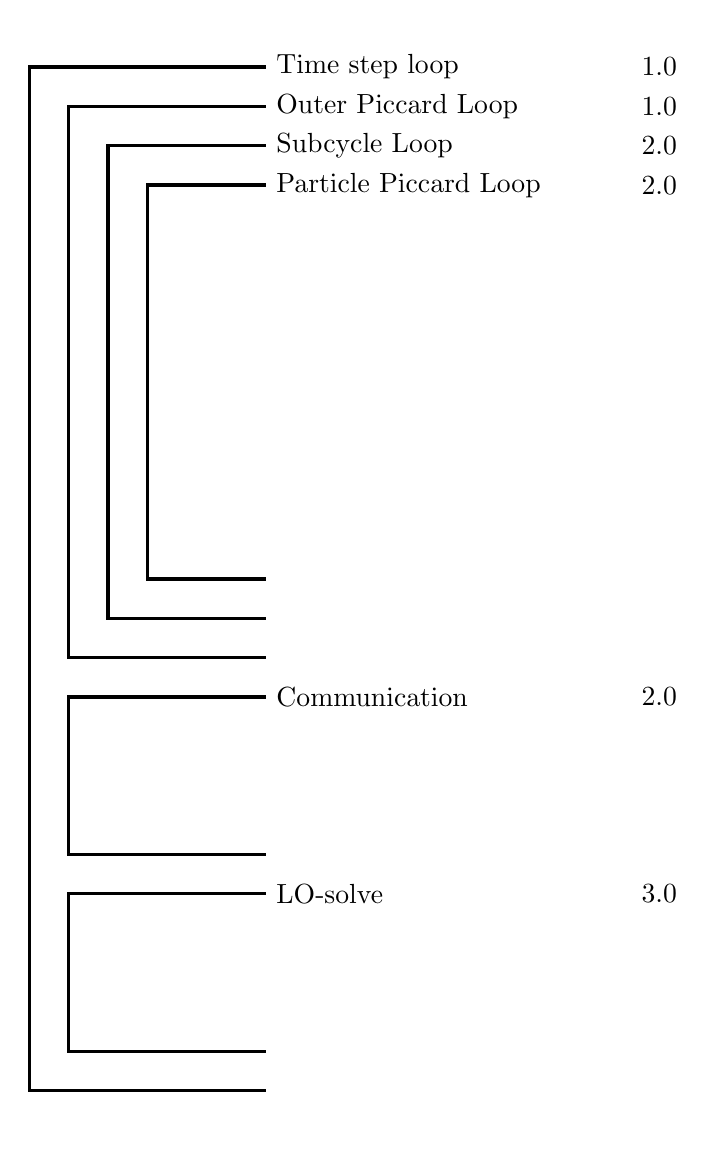
\begin{tikzpicture}
		\tikzstyle{every path}=[very thick]
		\tikzstyle{MainSty}=[->,dashdotted]
		\tikzstyle{CollSty}=[->,color=Emerald,densely dashdotted]
		\tikzstyle{ReinSty}=[->,color=Maroon,dashed]

		\edef\sizetape{1.0cm}
		\tikzstyle{tmtape}=[  minimum height=1.0cm,
								  text width=4cm,
								  align=left]

\def\ArrayA{1.0}
\def\ArrayB{1.0}
\def\ArrayC{2.0}
\def\ArrayD{2.0}
\def\ArrayE{2.0}
\def\ArrayF{3.0}

\newcommand*{\pshiftmm}{(-2.0mm,-2.0mm)}
\newcommand*{\pshiftpm}{(2.0mm,-2.0mm)}
\newcommand*{\pshiftmp}{(-2.0mm,2.0mm)}
\newcommand*{\pshiftpp}{(2.0mm,2.0mm)}




\node[tmtape] (tstep_loop) {Time step loop};
\node[tmtape,yshift=-5mm] at (tstep_loop) (opiccard) {Outer Piccard Loop};
\node[tmtape,yshift=-5mm] at (opiccard) (subcycle) {Subcycle Loop};
\node[tmtape,yshift=-5mm] at (subcycle) (ppiccard) {Particle Piccard Loop};
\node[tmtape,yshift=-6.5cm] at (ppiccard) (communication) {Communication};
\node[tmtape,yshift=-2.5cm] at (communication) (solve) {LO-solve}; 

\node[tmtape,yshift=-2cm] at (solve) (solve_end) {};
\node[tmtape,yshift=-5mm] at (solve_end) (tstep_end) {};
\node[tmtape,yshift=5mm] at (solve) (comm_end) {};
\node[tmtape,yshift=5mm] at (communication) (opiccard_end) {};
\node[tmtape,yshift=5mm] at (opiccard_end) (subcycle_end) {};
\node[tmtape,yshift=5mm] at (subcycle_end) (ppiccard_end) {};

\loopbracket{tstep_loop}{tstep_end}{3cm}
\loopbracket{solve}{solve_end}{2.5cm}
\loopbracket{communication}{comm_end}{2.5cm}
\loopbracket{opiccard}{opiccard_end}{2.5cm}
\loopbracket{subcycle}{subcycle_end}{2.0cm}
\loopbracket{ppiccard}{ppiccard_end}{1.5cm}


\node[xshift=5cm] at (tstep_loop.west) (timingnum1) {};
\node[xshift=5cm] at (opiccard.west) (timingnum2) {};
\node[xshift=5cm] at (subcycle.west) (timingnum3) {};
\node[xshift=5cm] at (ppiccard.west) (timingnum4) {};
\node[xshift=5cm] at (communication.west) (timingnum5) {};
\node[xshift=5cm] at (solve.west) (timingnum6) {};

\foreach \i/\Array in {1/\ArrayA,2/\ArrayB,3/\ArrayC,4/\ArrayD,5/\ArrayE,6/\ArrayF}
{
  \begin{scope}[start chain=1,node distance=1cm]
    \foreach \j in \Array
    {
      \node[on chain=1] at (timingnum\i) (n\i\j) {$\j$};
    }
  \end{scope}
}


\end{tikzpicture}
\end{document}

